\documentclass[10pt,a4paper]{article}

\usepackage[top=30pt,bottom=30pt,left=48pt,right=46pt]{geometry}
\usepackage{graphicx}
\usepackage{graphics}
\usepackage{amssymb}
\usepackage{epstopdf}
\usepackage{caption}
\usepackage{tipx}
\usepackage{tipa}
\usepackage{breakcites}
\usepackage{enumitem}
\usepackage{float}
\usepackage{color}
\usepackage[fleqn]{amsmath}
\usepackage[T1]{fontenc}
\usepackage[utf8]{inputenc}
\usepackage{authblk}
\usepackage{booktabs}
\usepackage{a4wide}


\title{Executive Summary: Applications of Natural Language Processing to Compare Shakespearean Sonnets to Modern Musical Artists}
\author[*]{Mariana Gonzalez Castro}
\author[*]{Carina Kalaydjian}
\author[*]{Dominique McDonald}
\author[*]{Angel Sierra}
\author[*]{DuoDuo Ying}
\affil[*]{Department of Statistics, UCLA}

\date{June 7, 2022}

\begin{document}

\maketitle

\section{Overview}

As a prominent music label, we care about artists that are truly outstanding and stand the trial of time. Out of 45 top artists, Amy Winehouse, Nickelback, and Cake are those artists due to the similarity between their work and Shakespeare's timeless sonnets. By leveraging Natural Language Processing algorithms, our label can predict future success based on the proven success of the past. 

\begin{table}[ht]
\centering
\resizebox{4cm}{2cm}{%
\begin{tabular}{lrrr}
  \hline
Artist & Overall Rank \\ 
  \hline
  amy-winehouse &   1\\ 
  nickelback &   2 \\ 
  cake &   3 \\ 
  adele &   4 \\ 
  joni-mitchell &  4 \\ 
  leonard-cohen &   6 \\ 
  paul-simon &  7\\ 
  blink-182 &  7\\ 
  bob-marley &  9 \\ 
  rihanna &  10 \\ 
   \hline
\end{tabular}%
}
\caption{Ranked Top 10 Most Similar Music Artist to Shakespeare} 
\label{tab:overallranktable}
\end{table}


\section{Methodology}

Before employing Natural Language Processing methods such as Keyword Extraction and Sentiment Analysis, we first obtained our data containing 154 Shakespeare's sonnets and songs of 45 modern top artists. The unit of observation is an artist and a subset of their discography. The data is stored on AWS RDS for portability.

\subsection{Keyword Extraction}

One of the NLP methods we used is Keyword Extraction. This algorithm returns the most frequently used keywords from Shakespeare and the 45 artists. Figure 1 provides an example of using Keyword Extraction to create a word cloud using the most used keyword by Shakespeare.

We compared the similarity between keywords for Shakespeare and the artists using first the number of similar words and then the Euclidean distance of frequency of these words. The result ranking is shown in Table 2.

\begin{table}
	\begin{minipage}{0.5\linewidth}
		\centering
		\resizebox{\columnwidth}{!}{%
		\begin{tabular}{lrrlr}
 		 \hline
			Word Rank & Artist & Word Count & Frequency & Keyword \\ 
 		 \hline
  			1 &  adele &   3 & 626.00 &  love time heart\\ 
  			2 &  nickelback &   3 & 11349.00 &  love time yet \\ 
  			3 &  bieber &   2 & 648.00 &  love time\\ 
  			4 &  dolly-parton &   2 & 685.00 &  love time \\ 
  			5 &  dj-khaled &   2 & 928.00 &  mine time \\ 
  			6 &  amy-winehouse &   2 & 3700.00 &  love time \\ 
  			7 &  bjork &   2 & 5341.00 &  love yet \\ 
  			8 &  leonard-cohen &   2 & 5972.00 &  love time \\ 
  			9 &  cake &   2 & 7690.00 &  love time \\ 
 			 10 &  paul-simon &   2 & 8464.00 &  love time \\ 
   		\hline
		\end{tabular}%	
		}
		\caption{Ranked Top 10 Most Similar Music Artist to Shakespeare Based on Keywords}
		\label{tab:wordranktable}
	\end{minipage}\hfill
	\begin{minipage}{0.45\linewidth}
		\centering
		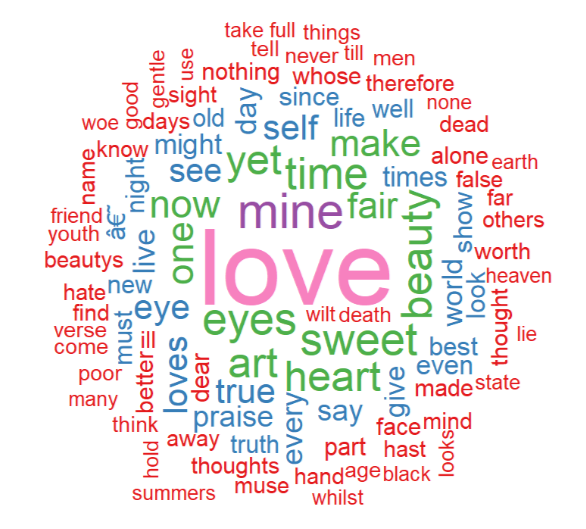
\includegraphics[width=5cm]{_assets/Shakespeare_Keywords_WordCloud.png}
		\captionof{figure}{Shakespeare Top Keywords Wordcloud}
		\label{ }
	\end{minipage}
\end{table}


%\begin{center}
%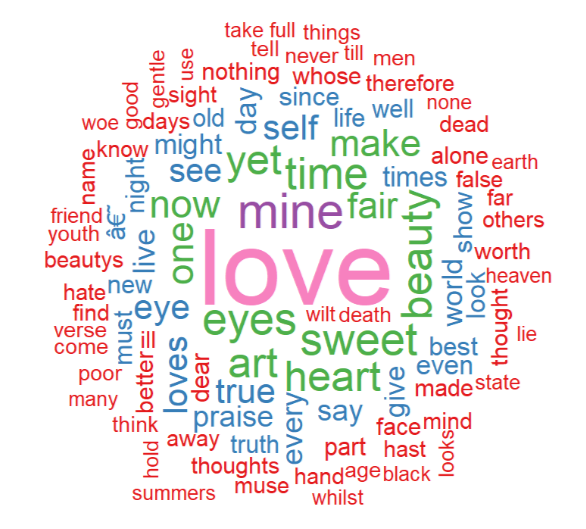
\includegraphics[width=12cm]{_assets/Shakespeare_Keywords_WordCloud.png}
%\end{center}

Based on this table, Adele, Nickelback and Bieber are the top 3 artists most similar to Shakespeare.

\subsection{Sentiment Analysis}

Another NLP method we used is Sentiment Analysis. More specifically, we analyzed Shakepeare's and artists' work using 8 emotions such as anger, anticipation, disgust, fear, joy, sadness, surprise, and trust to observe similarities and differences. Using k means clustering with 10 clusters, we observed clear trends between the artists:

\begin{center}

\includegraphics[width=10cm]{_assets/ClusterAnalysis_Fit10.png}
\captionof{figure}{Cluster Analysis using 8 Emotions from 45 Artists and Shakespeare}
\end{center}

Using Euclidean distance on the proportion of emotions, we found that Shakespeare's emotions through sonnets are most similar to the following artists:

   
\begin{table}[ht]
\centering
\resizebox{6cm}{1.7cm}{%
\begin{tabular}{lrr}
  \hline
Artist & Sent. Euclidean Distance & Sentiment Rank \\ 
  \hline
amy-winehouse & 0.001227 &       1 \\ 
  eminem & 0.001237 &       2 \\ 
  cake & 0.001304 &       3 \\ 
  nirvana & 0.001365 &       4 \\ 
  bob-dylan & 0.001471 &       5 \\ 
  bob-marley & 0.001492 &       6 \\ 
  johnny-cash & 0.001589 &       7 \\ 
  nickelback & 0.001827 &       8 \\ 
  britney-spears & 0.002097 &       9 \\ 
  rihanna & 0.002249 &      10 \\ 
   \hline
\end{tabular}%
}
\caption{Ranked Top 10 Most Similar Music Artist to Shakespeare Based on Sentiments} 
\label{tab:wordranktable}
\end{table}



Based on this table, Amy Winehouse, Eminem, and Cake are the top 3 artists most similar to Shakespeare based on sentiment.

\section{Results}

Combining the rankings obtained by Keyword Extraction and Sentiment Analysis, our final ranking is following:

\begin{table}[ht]
\centering
\resizebox{8cm}{2cm}{%
\begin{tabular}{lrrr}
  \hline
Artist & Word Rank & Sentiment Rank & Overall Rank \\ 
  \hline
amy-winehouse &   6 &   1 &   7 \\ 
  nickelback &   2 &   8 &  10 \\ 
  cake &   9 &   3 &  12 \\ 
  adele &   1 &  21 &  22 \\ 
  joni-mitchell &  11 &  11 &  22 \\ 
  leonard-cohen &   8 &  15 &  23 \\ 
  paul-simon &  10 &  22 &  32 \\ 
  blink-182 &  18 &  14 &  32 \\ 
  bob-marley &  27 &   6 &  33 \\ 
  rihanna &  25 &  10 &  35 \\ 
   \hline
\end{tabular} %
}
\caption{Ranked Top 10 Most Similar Music Artist to Shakespeare} 
\label{tab:overallranktable}
\end{table}


We show that Amy Winehouse, Nickelback, Cake, Adele, and Joni Mitchell are top 5 closest with Shakespeare using the two NLP methods. More interesting findings include:

\begin{itemize}

\item Despite being number one on keyword, Adele was listed 21 closest artists to Shakespeare in terms of sentiment, therefore Adele was not amongst top 3 closest artists to Shakespeare in the final ranking.
\item Using Sentiment Analysis, we compared emotions such as anger, anticipation, disgust, fear, joy, sadness, surprise, and trust within the sonnets and songs. We found that Bob Dylan is one of the closest in emotions with Shakespeare. Dylan was also the first musician to win Nobel Prize in Literature "for having created new poetic expressions within the great American song tradition". [Wikipedia]

\end{itemize}


\section{Limitations \& Recommendations}
\begin{itemize}

\item The R package for analyzing sentiment offers different results when collapse the sonnets into a single corpus vs not collapsing the sonnets. We would get more accurate results not collapsing, but more consistent result collapsing. In this case, we collapsed all the sonnets into one single corpus, but recognize that the result might differ if we analyze sonnets and songs without collapsing.
\item The 45 artists we chose are already outstanding. Therefore, we could look into each individual songs or more artists to derive further results.
\item Shakespeare’s language usage is different from the modern day language, and we would improve our result using modern translation of Shakespeare's sonnets.

\end{itemize}



\end{document}
